\documentclass[12pt,oneside,letterpaper]{article}
\usepackage{longtable}
\usepackage{graphicx}
\usepackage[nogroupskip]{glossaries}
\usepackage{hyperref}
%\usepackage{fullpage}

\newenvironment{packed_enumerate}{ %custom enumerate for single-spacing
\vspace{-7mm}
\begin{enumerate}
  \setlength{\itemsep}{0pt}
  \setlength{\parskip}{0pt}
  \setlength{\parsep}{0pt}
}{\end{enumerate}
\vspace{-8mm}}

\pagestyle{headings}
\oddsidemargin 0.25in \textwidth     6.25in \topmargin     0.4in
\textheight    8.5in


%This is for adding things to the glossary. Will Automatically be alphabetical order.
% NOTE: IN ORDER FOR THE ITEM TO APPEAR IN GLOSSARY, YOU MUST USE "\gls{[name of entry]}" so that the glossary can put a page number of where it is. the sort needs to be the first letter or so of the name of the entry -- or the entire word if need be for ordering
\newglossaryentry{example}
{ name=test entry,
  description={This is the definition of the word},
  sort={0}
  }
  
\newglossaryentry{front end}
{ name=front end,
  description={a client which is usually a device or service that is used to communicate between the user and the system's database or logic (back end)},
  sort={f}
}
  
\newglossaryentry{back end}
{ name=back end,
  description={the database or logic of a system, often is not directly accessible by the user},
  sort={b}
}
  
\newglossaryentry{Firebase}
{ name=Firebase,
  description={Google's cloud service that provides a realtime database and \gls{back end}. The service provides application developers an API that allows application data to be synchronized across clients and stored on Firebase's cloud},
  sort={f}
}

\newglossaryentry{AWS}
{ name=AWS,
  description={Amazon Web Services: a secure cloud services platform, offering compute power, database storage, content delivery and other functionality to help businesses scale and grow},
  sort={a}
}

\newglossaryentry{S3}
{ name=S3,
  description={Simple Storage System: Storage of files and information on the cloud. Part of AWS},
  sort={s}
}


\makenoidxglossaries


\begin{document}


\title{\bfseries Data Classifier: \\
Software Requirements Specification\\
Version 2.2}

\author {
\large{Team Mark}\\
\emph{Computer Science Department}\\
\emph{California Polytechnic State University}\\
\emph{San Luis Obispo, CA USA}\\
}

\date{November 1, 2018}
\maketitle \thispagestyle{empty}

\pagebreak
\tableofcontents

\addcontentsline{toc}{section}{Revision History}

\addcontentsline{toc}{section}{Credits}

\section*{Credits}
\begin{tabular}{|l|l|p{2.5in}|l|}
\hline
\textbf{Name}&\textbf{Date}&\textbf{Role}&\textbf{Version}\\
\hline
Geraldo Macias&October 9, 2018&Lead Author of Other Nonfucntional Requirements&1.0\\
\hline
Matt Yarmolich&October 9, 2018&Lead Author of System Features&1.0\\
\hline
Spencer Schurk&October 10, 2018&Lead Author of Introduction&1.0\\
\hline
Jake Veazey&October 10, 2018&Maintains Document and glossary. Assisted on \gls{front end} System Features&1.0\\
\hline
Brad Foster&October 10, 2018&Lead Author of Overall Description&1.0\\
\hline
&&&\\
\hline
\end{tabular}

\section*{Revision History}
\begin{tabular}{|l|l|p{2.5in}|l|}
\hline
\textbf{Name}&\textbf{Date}&\textbf{Reason for Changes}&\textbf{Version}\\
\hline
Geraldo Macias&October 8, 2018&Completion of Other Nonfunctional Requirements&1.0\\
\hline
Spencer Schurk&October 10, 2018&Addition of my User Persona, Use Case, Functional Requirement, and Non-Functinal Requirement&1.0\\
\hline
Jake Veazey&October 10, 2018&Addition of \gls{front end} system reqs, Use Case, User Persona, clean up/add glossary&1.0\\
\hline
Spencer Schurk&October 10, 2018&Completion of Introduction&1.0\\
\hline
Brad Foster&October 10, 2018&Completion of Overall Description&1.0\\
\hline
Geraldo Macias&October 24, 2018&Section 6 verified, User Description update, Use Case 6 update&2.0\\
\hline
Spencer Schurk&October 24, 2018&Section 1 revisions&2.0\\
\hline
&&&\\
\hline
Jake Veazey&October 24, 2018&Clarification and additions to Overall Description, Glossary, and overall maintenance of the document&1.0\\
\hline
Spencer Schurk&October 30, 2018&Modification to use case 2&2.1\\
\hline
Geraldo Macias&December 10, 2018&Various fixes for 2.2&2.2\\
\hline
&&&\\
\hline
\end{tabular}

\newpage

\section{Introduction}
\subsection{Purpose}
The purpose of this document is to present the functional and non-functional requirements of our Data Classification application version 1.0. In addition, it also features potential user personas, fully-dressed use cases of the product, and diagrams to complement text descriptions. This document serves as a source of reference and guidance during the development process. Please note, this document does not describe the architecture of this application.

\subsection{Document Conventions}
Requirements listed in later sections will adhere to the following convention: FR-n for functional requirements, and NR-m for non-functional requirements, where n and m is the requirement's numerical value. No two functional requirements shall have the same n-value, and likewise, no two non-functional requirements shall have the same m-value.

\subsection{Intended Audience and Reading Suggestions}
This document was intended for and targeted at the following parties.
\subsubsection{Developers}
Developers of this project will use this document as a reference during the development process. Specifically, the Use Cases and Functional Requirements should be referenced the most.\newline
\textit{Suggested Reading Order}\newline
\begin{packed_enumerate}
\item Overall Description
\item System Features
\item Functional Requirements
\item Non-Functional Requirements\newline
\end{packed_enumerate}

\subsubsection{Customer - Mark Logic}
Our customers at Mark Logic will use this document to make sure we're on track with the project and have the correct vision. They will be able to verify our requirements are applicable to the product they want us to produce.\newline
\textit{Suggested Reading Order}\newline
\begin{packed_enumerate}
\item Overall Description
\item User Cases
\item External Interface Requirements
\item Non-Functional Requirements\newline
\end{packed_enumerate}

\subsubsection{Supervisor - Bruno Da Silva}
Bruno Da Silva, the team's professor in CPE 402, will read this document to understand how we view the project. Additionally, he will use this document to verify the team will remain up to date with changes, and that the team will update this document.\newline
\textit{Reading Suggestion}\newline
\par Bruno Da Silva should thoroughly read this document to ensure our team has an acceptable level of understanding of the class material.
\subsection{Project Scope}
For information regarding the scope and vision of this project, please reference the team's \textit{\underline{Vision and Scope}} document.\newline\newline
\url{https://github.com/rocketeer55/CSC402-GENERAL/blob/master/VisionAndScope.pdf}


\section{Overall Description}
\subsection{Product Perspective}
One of the biggest unsolved roadblocks for data scientists is data sanitization and grooming. Data scientists spend excessive amounts of time preparing data before even being able to do productive work. Eliminating this downtime would allow more room for data scientists to do the meaningful work that they actually want to do. Our application aims to do just this. Through the use of machine learning techniques and a robust web interface, our application will take various ungroomed data sets as input and will convert them into cohesive, organized documents as output. We want to make the process of pre-analysis data grooming as automated and painless as possible. 
\newline The classification service will be composed of two parts: a \gls{back end} that contains machine learning and connection to databases and storage technology and a \gls{front end} that links the \gls{back end} to the user. The overall scope of the \gls{back end} will be to take any number of inputted, ungroomed, files, classify using machine learning and algorithms, and use services and databases to store user inputted information and any output that relates to the user's input. The \gls{front end} takes on the role of the link from user to backend and will, overall, allow user uploads of files and user downloads of the \gls{back end}s output. 
\subsection{Product Features}
The primary feature of the application is that it will be able to take data from various different "silos" and automatically make meaningful, organized categories out of them. The program will be robust enough to make sense out of data that is unconventionally or even improperly formatted. The application will also have a web interface that data scientists will be able to interact with.
\subsection{User Personas}
\subsubsection{Frank McLaughlin}
\textbf{Author}: Spencer Schurk\newline
\textbf{Age}: 24\newline
\textbf{Job}: Data Scientist\newline
\textbf{Bio}:\newline
\par Frank McLaughlin is a 24 year old data scientist working for a large e-Sports company. Frank has been interested in video games from a very young age, and this interest has helped shape his life and influence his friends. His parents never appreciated his video game obsession, but Frank didn't let that stop him.
\par Frank graduated from UC Irvine with a bachelor's degree in Computer Science. After graduating, Frank worked at a startup for a delivery app. He was assigned data analysis tasks, but they were very basic. Frank did not like this job at the startup very much, as he felt it was too fast paced with very little organization. Everbody was stepping on everyone else's feet. Eventually, it was time for Frank to find a new job.
\par Frank then found a job at a major e-Sports company. Here, he was also hired as a data analyst. He likes working at this new company a lot better, since they use better tools and he can be more efficient. However, the data sets Frank works with now are much larger. He hates manually searching through tables to find the correct data types for his tasks.
\par Luckily, Frank has heard that his e-Sports company will soon be using a new tool to automatically classify the data in these data sets. He believes this will instantly help him be more efficient, and get more data analysis done quicker. Now, Frank can go home sooner and play more video games.\newline

\subsubsection{Dave Fuego}
\textbf{Author}: Matt Yarmolich\newline
\textbf{Age}: 25\newline
\textbf{Job}:Sports Data Analyst\newline
\textbf{Bio}:\newline
\par Brian Fuego is a 25 year old Sports Data Analyst working for the Seattle Seahawks. He
has been an avid sports fan for his entire life and loves following the numbers and figuring out threats on the field for his team. His dad really wanted him to be a football player, but he was never good enough to play on any competitive team.
\par Thanks to his father?s drive, he has been able to push himself into fields that he believed would make his father proud. Thus he began a career as a data analyst for his dad (and his) favorite sports team. Unfortunately, Dave is getting sick of doing his job week by week and wants tools to help make his job go by faster so he has more time doing his actual passion, coding.
\par Through his relentless search for tools, Dave has found the data classifier with a GUI that helps make his job way easier. He likes that it uses the newest trends in computing (machine learning) and that it has GUI for ease of use to make his job go by faster. Dave plans on implementing this technology so that he has more time to do his passion and work on creating games written in OpenGl and c++ since that is his bread and butter and what he likes doing the most in this world.\newline

\subsubsection{Bread Feuyser}
\textbf{Author}: Brad Foster\newline
\textbf{Age}: 27\newline
\textbf{Job}:Music Data Analyst\newline
\textbf{Bio}:\newline
\par Bread Feuyser is a 27 year old Music Data analyst working for a major record label. Bread has been a passionate music fan for his entire childhood, adolescence, and adult life. He found his way into the music data industry when he realized that he had an unusual ability to make sense out of seemingly meaningless and nonsensical data. 
\par Bread is a Third Degree Supreme-Master class data analyst, but has trouble listening to music while grooming data during the pre-analysis phase. Any sort of mis-classification or other kind of organizational mistake completely throws off his rhythm. This consequently adversely affects his ability to "connect" with the music he is listening to, which ultimately leads to drastic reductions in his productivity. Bread's main strength is his ability to make wild and unconventional connections between musical data sets, and this ability is fueled by his unrivaled love for "sick beats" and "clean mixes" (sic).
\par Seeming as though The Hand of God reached down and personally delivered it to him, Bread one day stumbled upon a data classifier that had the perfect set of features to solve all of his data problems. It allowed him to feed it various disorganized data sets and turn them into a single, cohesive, analysis-ready database. It even had a web based interface with buttons that Bread could click in sync with the music he was listening to. The musical world will continue to be changed, though now at an even faster rate, by Bread's groundbreaking discoveries.\newline

\subsubsection{Chad Chaderson}
\textbf{Author}: Jake Veazey\newline
\textbf{Age}: 19\newline
\textbf{Job}:Data Company Intern\newline
\textbf{Bio}:\newline
\par Chad Chaderson is a Computer Science student, with a minor is data science, at Yale University and began working for a data analyst company the summer after his second year of school. Chad does not know much of what he wants to do with his degrees after college, so he is using the internship as a way to expand his horizons to learn and discover. 
\par At this internship Chad has been asked to do a lot of chores that the rest of the employees don't want to do. One such task has been to take many files of data that has not been classified into its categories but had no way to do so in a fast and easy way. After a few weeks of manually sorting and classifying data from multiple files that we assigned to him, Chad got frustrated and was contemplating leaving the company and changing his area of concentration. Before he made the decision, Chad, spoke to his boss and learned that there are tools online that may be able to assist him in his work -- this is when Chad found the Data Classifier tool and online GUI.
\par Chad found that the entire system worked well with his company's information, and because of his excellent work, he got an offer to come back the following summer.

\subsubsection{Davide Falessi}
\textbf{Author}: Landon Gerrits\newline
\textbf{Age}: 37\newline
\textbf{Job}:Project Manager\newline
\textbf{Bio}:\newline
\par Davide is 37 year old project manager from Italy. He works for a data analysis company, Matthew Reason. Davide is a good project manager, in fact he's highly technical. He began his career and a software engineer specifically working in data science. He now is a project manager for the data science division of his company. Davide interfaces often interfaces with the business of the company. The business often asks Davide to provide high level data sheets that show the final output of Davide's team's classification algorithms.
\par Last year, Matthew Reason had many clients from the sports industry, specifically soccer. Many major news networks contacted Matthew Reason to analyze and filter their data based around player statistics. Davide's team was tasked with creating a program that could rapidly classify and sort this player data.
\par Davide's team was underfunded to have enough man power to create this program. Davide's team was already working on 4 other important projects for the company. While researching this problem, he found a data classifier that did exactly this. Davide purchased this program and it was downloaded and installed in a matter of minutes. Davide read the documentation and imported a data set with player stats. He ran the program and moments later he received an output file that classified player names, countries, and many other valuable classifications. Davide showed this to the business and they were thrilled that he was able to get these data classifications with such a short turnaround.


\subsubsection{Mantis Tobaggon}
\textbf{Author}: Geraldo Macias\newline
\textbf{Age}: 60\newline
\textbf{Job}:Financial Investor\newline
\textbf{Bio}:\newline
\par Mantis was a failing financial investor who always seemed to be a little bit behind the trends on Wall Street. He tried using different brokering companies but their rates were beyond reasonable. After doing a little research Mantis started to see the buzz statement Data Science in multiple places. This looked like a lot of work to get into, but this was the answer Mantis has been looking for. 
\par For one year Mantis spent time on Udemy taking various online classes learning how to maximize the effectiveness of Scikit learn.Because Mantis has not taken any formal computer science courses he doesn't really understand coding outside of data science.After taking his year of Udemy courses Mantis became a power house of an investor on Wall Street but he quickly became bored with the market. With laws changing about sports betting, Mantis saw this as an opportunity to move into the sports industry.
\par There is a lot of public available datasets  of sports statistics but due to Mantis' inexperience in computer science, he is unable to manage and quickly organize all his data. This is becoming a major problem for Mantis and is now looking for a solution to manage all his data so he can spend more time analyzing data and making money.


\newpage
\subsection{User Classes and Characteristics}
\begin{longtable}{|r|p{3.8in}|}
\hline
\textbf{User Class}&\textbf{Description}\\
\hline
Developer&The Developer will design, implement,\newline test, and maintain the application.\\
\hline
Data Scientist with programming knowledge&A Data Scientist that will require\newline advanced technical features from \newline the application.\\
\hline
Data Scientist without programming knowledge&A Data Scientist that will require\newline a simplistic interface and feature set \newline from the application.\\
\hline
\end{longtable}
\subsection{Operating Environment}
The program will exist as a web based application with a React \gls{front end}, Flask \gls{back end} as well as an s3 database and a block storage system. The data classifier will be written in Python.
\subsection{Design and Implementation Constraints}
The \gls{back end}/machine learning parts of the application will have to be written in Python coupled with the Scikit Learn. Our application also must implement a web based interface that will be written in JavaScript that will call APIs built in the \gls{back end}.
\subsection{User Documentation}
During implementation, we will be monitoring issues through the use of JIRA. We will likely intend to include some simple documentation for using the user interface along with the application. 
\subsection{Assumptions and Dependencies}
We are assuming that we will easily be able to integrate a database solution (i.e. MongoDB, DynamoDB) into our application during development. In addition, when using data with columns, our machine learning algorithm will use Linear SVC. If this process fails we will use Naive Bayes. For data without column names we will use K-Means, Spectral clustering, and GMM in that order. \gls{AWS} has also been made available for us to use and can be nicely integrated with the \gls{back end} to store files in \gls{S3} Buckets and other information in one of the offered databases. Finally, we are assuming that we will be able to use something like Google Firebase for our web app development.


\section{Use Cases}

\subsection{\label{Selecting the Proper Classification from the UIl}Use Case 1: Select Proper Classification Category}
This use case details the the path of the data analyst providing feedback to the machine learning algorithm written by Matt Yarmolich

\begin{longtable}{|r|p{3.8in}|}
\hline
Use Case ID:&1\\
\hline
Use Case Name:&Select Proper Classification Category\\
\hline
Created By:&Matt Yarmolich\\
\hline
Last Updated By:&Matt Yarmolich\\
\hline
Date Created:&October 9, 2018\\
\hline
Date Last Updated:&October 9, 2018\\
\hline
Actors:&Data Analyst\\
\hline
Description:&A Data Analyst accesses the data classification \gls{front end} by feeding it information from an HTML-5 input tag and having the information parsed by the system. .\\
\hline
Preconditions:&
\begin{packed_enumerate}
\item the Data Analyst is logged into the system.
\item the Data Analyst is a registered user for the system.
\item the Data Analyst has a dataset that needs to be analyzed.
\end{packed_enumerate}\\
\hline
Postconditions:&
\begin{packed_enumerate}
\item the dataset has been correctly parsed by the data classifier
\item the classifier has outputted a variety of tags for verification by the Data Analyst. 
\item the Data Analyst is capable of correctly identifying the dataset
\end{packed_enumerate}\\
\hline
Normal Flow:&1.0 Select the correct category from the data classifier\\
&  %line needed for aligning enumeration 
\begin{packed_enumerate}
\item The Data Analyst uploads the dataset to the \gls{front end} of the system
\item System displays upload status
\item System displays upload complete and feeds the data to the \gls{back end}
\item the \gls{back end} outputs the results of the data in a web-parsable format (JSON)
\item The \gls{front end} parses this output and displays it to the data analyst along with the columns in question
\item System displays upload complete and feeds the data to the backend
\item The machine learning classifier classifies the initial column data
\item The machine learning classifier the rest of the data based on past data columns and previous data fed through the system
\item the backend outputs the results of the data in a web-parsable format (JSON)
\item the Data Analyst reviews the data and selects the correct category based on their domain knowledge
\item The \gls{front end} feeds their result back to the data classification \gls{back end}
\item System displays the correct tagging of the data set
\end{packed_enumerate}\\
\hline
Alternative Flows:&1.1 No results from \gls{back end} (branch after step )\\
&  %line needed for aligning enumeration 
\begin{packed_enumerate}
\item The system outputs no previously learned categories
\item The Data Analyst inputs a new category for the data set
\item Return to step 8.
\end{packed_enumerate}\\
\hline
Alternative Flows:&1.2 The Data Analyst wants to rename a dataset\\
&  %line needed for aligning enumeration 
\begin{packed_enumerate}
\item The Data Analyst clicks the button to edit the name of a data set
\item The Data Analyst inputs a new name for the data set
\item The Data Analyst clicks confirm
\item Return to step 8.
\end{packed_enumerate}\\

Exceptions:&1.0.E.1 System loses connection to front end(at step 1)\\
&1. 	System informs Data Analyst that connection has been lost to the server\\
&2.	Patron reloads page\\
&3.	System restarts use case.\\
\hline
Includes:&None\\
\hline
Priority:&High\\
\hline
Frequency of Use:&Approximately n uses per data set (depends on column inputted)\\
\hline
Business Rules:&TBD\\
\hline
\end{longtable}


\subsection{\label{Upload Data Sets}Use Case 2: Upload Data Sets}
This use case details the the user flow of uploading data sets to the data classifier using the web interface, written by Spencer Schurk.

\begin{longtable}{|r|p{3.8in}|}
\hline
Use Case ID:&2\\
\hline
Use Case Name:&Upload Data Sets\\
\hline
Created By:&Spencer Schurk\\
\hline
Last Upadted By:&Spencer Schurk\\
\hline
Date Created:&October 10, 2018\\
\hline
Date Last Updated:&October 10, 2018\\
\hline
Actors:&Data Analyst\\
\hline
Description:&After logging in, the system allows a data analyst to upload multiple data sets. After uploading data sets, the data analyst can begin the classification process.\\
\hline
Preconditions:&\begin{packed_enumerate}
\item The data analyst is logged into the system.
\item The data analyst has not uploaded any data sets.
\item The data analyst has not began the classification process.
\end{packed_enumerate}\\
\hline
Postconditions:&\begin{packed_enumerate}
\item All selected data sets have been uploaded.
\item The data analyst is now able to begin the classification process.
\end{packed_enumerate}\\
\hline
Normal Flow:&1.0 Select multiple files to upload.\newline
\begin{packed_enumerate}
\item The data analyst selects "Upload Files" button.
\item System opens local machine's file explorer / file selector.
\item Data analyst selects multiple files from their local machine.
\item Data analyst selects "Ok" or "Upload" on system file explorer.
\item System displays list of files selected and begins to upload files.
\item System allows user to edit name of file being uploaded.
\item System displays progress of each file being uploaded.
\item System displays "Upload successful" message after upload completes.
\item Data analyst selects "Begin Classification" button.
\end{packed_enumerate}\\
\hline
Alternate Flows:&1.1 Select files more than once. (branch after step 4)\newline
\begin{packed_enumerate}
\item While previously selected files are uploading, data analyst selects "Upload more files"
\item System opens local machine's file explorer / file selector.
\item Data analyst selects multiple files from their local machine.
\item Data analyst selects "Ok" or "Upload" on system file explorer.
\item System adds selected files to list of previously selected files that are uploading.
\item Flow continues on step 8 of normal flow
\end{packed_enumerate}\\
\hline
Exceptions:&1.0.E.1 Data analyst uploads unsupported file. (at step 4)\newline
\begin{packed_enumerate}
\item System displays error message, with file name present.
\item Data analyst selects "OK" button.
\item System removes selected file from list of files to upload.
\item System continues to upload other selected files.\newline
\end{packed_enumerate}
1.0.E.2 Upload fails for any reason. (at step 5)\newline
\begin{packed_enumerate}
\item System displays "Upload failed" message
\item Data analyst selects "Try again" or "Cancel" button.
\item If "Try again" is selected, system continues at step 5, with all progress at 0.
\item If "Cancel" button selected, page is refreshed, and continues at step 1.
\end{packed_enumerate}\\
\hline
Includes:&None\\
\hline
Priority&High\\
\hline
Frequency of Use:&Once per data classification process.\\
\hline
Business Rules:&TBD\\
\hline
Special Requirements:&TBD\\
\hline
Assumptions:&\begin{packed_enumerate}
\item Data sets are locally stored on data analyst's machine.
\item Data analyst has active internet connection capable of uploading files.
\end{packed_enumerate}\\
\hline
Notes and Issues:&\begin{packed_enumerate}
\item What if the data analyst uploads the wrong file?
\end{packed_enumerate}\\
\hline
\end{longtable}

\subsection{\label{Log In}Use Case 3: Log In}
This use case details the flow of logging into the application, written by Brad Foster.

\begin{longtable}{|r|p{3.8in}|}
\hline
Use Case ID:&3\\
\hline
Use Case Name:&Log In\\
\hline
Created By:&Brad Foster\\
\hline
Last Upadted By:&Brad Foster\\
\hline
Date Created:&October 10, 2018\\
\hline
Date Last Updated:&October 10, 2018\\
\hline
Actors:&Data Analyst\\
\hline
Description:&The user must log into their account before accessing the app's features.\\
\hline
Preconditions:&\begin{packed_enumerate}
\item The data analyst is not logged into the system.
\item The data analyst has the application open.
\end{packed_enumerate}\\
\hline
Postconditions:&\begin{packed_enumerate}
\item The data analyst is now logged in.
\end{packed_enumerate}\\
\hline
Normal Flow:&1.0 Log In Successfully.\newline
\begin{packed_enumerate}
\item The data analyst opens the application.
\item System prompts the user for their username and password.
\item Data analyst inputs their username and password.
\item System verifies their credentials.
\item System displays the application's main screen.
\end{packed_enumerate}\\
\hline
Alternate Flows:&1.1 Log in Failed (branch after step 3)\newline
\begin{packed_enumerate}
\item System detects that there is a mistmatch between username and password.
\item System displays an appropriate error.
\item System prompts the user for their username and password again.
\end{packed_enumerate}\\
\hline
Includes:&None\\
\hline
Priority&High\\
\hline
Frequency of Use:&Once per launch of the application.\\
\hline
Business Rules:&TBD\\
\hline
Special Requirements:&TBD\\
\hline
Assumptions:&\begin{packed_enumerate}
\item Account credentials can be securely stored.
\end{packed_enumerate}\\
\hline
Notes and Issues:&TBD\\
\hline
\end{longtable}

\subsection{\label{Log In}Use Case 4: Log Out}
This use case details the flow of logging out of the application, written by Brad Foster.

\begin{longtable}{|r|p{3.8in}|}
\hline
Use Case ID:&4\\
\hline
Use Case Name:&Log Out\\
\hline
Created By:&Brad Foster\\
\hline
Last Upadted By:&Brad Foster\\
\hline
Date Created:&October 10, 2018\\
\hline
Date Last Updated:&October 10, 2018\\
\hline
Actors:&Data Analyst\\
\hline
Description:&The user must log out of their account once they are done using the application.\\
\hline
Preconditions:&\begin{packed_enumerate}
\item The data analyst is logged into the system.
\item The data analyst has the application open.
\end{packed_enumerate}\\
\hline
Postconditions:&\begin{packed_enumerate}
\item The data analyst is now logged out.
\item The System is now showing the log in screen.
\end{packed_enumerate}\\
\hline
Normal Flow:&1.0 Log Out Successfully.\newline
\begin{packed_enumerate}
\item The data analyst clicks the log out button.
\item The user's uploaded/categorized datasets are stored to a database.
\item System closes the main screen and displays the log in screen.
\item System displays a successful log out message.
\end{packed_enumerate}\\
\hline
Includes:&None\\
\hline
Priority&High\\
\hline
Frequency of Use:&Once per login session.\\
\hline
Business Rules:&TBD\\
\hline
Special Requirements:&TBD\\
\hline
Assumptions:&TBD\\
\hline
Notes and Issues:&TBD\\
\hline
\end{longtable}





\subsection{\label{Upload Data Sets}Use Case 4: Viewing the Classifier Logs}

\begin{longtable}{|r|p{3.8in}|}
\hline
Use Case ID:&4\\
\hline
Use Case Name:&Upload Data Sets\\
\hline
Created By:&Jake Veazey\\
\hline
Last Updated By:&Jake Veazey\\
\hline
Date Created:&October 10, 2018\\
\hline
Date Last Updated:&November 1, 2018\\
\hline
Actors:&Data Analyst\\
\hline
Description:&After logging in, the system allows a data analyst to upload multiple data sets. After uploading data sets, the data analyst can begin the classification process. Each step of the classification process will be noted and time logged. The Logs page will provide original input and classified output for all data sets uploaded.\\
\hline
Preconditions:&\begin{packed_enumerate}
\item The data analyst is logged into the system.
\item The data analyst has just uploaded a data set and identied the set with a name or ID
\item The data analyst has just begun the classification process.
\end{packed_enumerate}\\
\hline
Postconditions:&\begin{packed_enumerate}
\item All selected data sets have been uploaded.
\item The classification process has been completed.
\item All uploaded data sets are displayed with outputs and timestamps in the logs.
\end{packed_enumerate}\\
\hline
Normal Flow:&1.0 Select multiple files to upload.\newline
\begin{packed_enumerate}
\item The data analyst uploads their data sets.
\item The data begins to be classified
\item As the data is going through classifications, each step is being logged to show user status
\item When the data is done being classified, the logs will have available the input, output, and status logs
\end{packed_enumerate}\\
\hline
Alternate Flows:&1.1 User uploads more than one file. (branch after step 4)\newline
\begin{packed_enumerate}
\item Each uploaded file will enter a queue
\item While queue is not empty, continue Normal Flow
\end{packed_enumerate}\\
Alternate Flows:&1.2 User replaces a file. (branch after step 1)\newline
\begin{packed_enumerate}
\item The previous file(s) will be deleted from the upload process and the new file(s) will take its place
\end{packed_enumerate}\\
Alternate Flows:&1.3 User cancels classification of file (branch after step 3)\newline
\begin{packed_enumerate}
\item The file(s) selected to stop will break out of the code they're being run through and display a "User Ended" message. Any other files not yet classified or stopped will continue classification.
\end{packed_enumerate}\\
\hline
Exceptions:&1.0.E.1 Data analyst uploads a supported file, but incompatible data. (at step 3)\newline
\begin{packed_enumerate}
\item While the data set(s) the user uploaded are being classified the process fails
\item This can be due to incompatible information or incorrect files
\item The logger will display the failed status and attempt to show the reason the classification failed.
\end{packed_enumerate}\\
\hline
Includes:&None\\
\hline
Priority&Medium\\
\hline
Frequency of Use:&Once per data classification process.\\
\hline
Business Rules:&TBD\\
\hline
Special Requirements:&TBD\\
\hline
Assumptions:&\begin{packed_enumerate}
\item Data sets are locally stored on data analyst's machine.
\item Data analyst has active internet connection capable of uploading files.
\end{packed_enumerate}\\
\hline
Notes and Issues:&\begin{packed_enumerate}
\item Check for all errors at each step in the classification process
\end{packed_enumerate}\\
\hline
\end{longtable}

\subsection{\label{Upload Data Sets}Use Case 5: Exporting data and logs}

\begin{longtable}{|r|p{3.8in}|}
\hline
Use Case ID:&5\\
\hline
Use Case Name:&Export Data\\
\hline
Created By:&Landon Gerrits\\
\hline
Last Updated By:&Landon Gerrits\\
\hline
Date Created:&October 10, 2018\\
\hline
Date Last Updated:&October 10, 2018\\
\hline
Actors:&Data Analyst and Project Managers\\
\hline
Description:&After the system has run and classified its data input, it is ready to be exported. Data analysts and project managers can choose to export this data to specified file types.\\
\hline
Preconditions:&\begin{packed_enumerate}
\item The user is logged into the system.
\item The user has uploaded a data set
\item The user has run the classification process.
\item The classification process has been completed.
\end{packed_enumerate}\\
\hline
Postconditions:&\begin{packed_enumerate}
\item All selected data sets have been uploaded.
\item The classification process has been completed.
\end{packed_enumerate}\\
\hline
Normal Flow:&1.0 Select expected file type output.\newline
\begin{packed_enumerate}
\item The user can view the classifications in the program's GUI
\item The user can select the specified file output type: .JSON, .CSV, .XML
\item The specified file output type is exported.
\end{packed_enumerate}\\
\hline
Alternate Flows:&1.1 User chooses multiple export file types\newline
\begin{packed_enumerate}
\item User runs the program
\item User checks multiple file types for export 
\item The system exports the selected file types. 
\end{packed_enumerate}\\
\hline
Exceptions:&1.0.E.1 Data analyst selects .CSV\newline
\begin{packed_enumerate}
\item User selects .CSV file type for export (Comma Separated Value documents do not work well with grouped sets the JSON and XML can handle)
\item User selects a location to put the file
\item The system exports a .zip file that contains a folder of .CSV files for each classification 
\end{packed_enumerate}\\
\hline
Includes:&None\\
\hline
Priority&Medium\\
\hline
Frequency of Use:&Once per data classification process.\\
\hline
Business Rules:&TBD\\
\hline
Special Requirements:&TBD\\
\hline
Assumptions:&\begin{packed_enumerate}
\item Data set is large enough to be classified (minimum several hundred entries)
\end{packed_enumerate}\\
\hline
Notes and Issues:&\begin{packed_enumerate}
\item Supporting multiple export file types will be time consuming for developers. A single file type may be desirable if there are higher priorities for the project
\end{packed_enumerate}\\
\hline
\end{longtable}

\subsection{\label{Upload Data Sets}Use Case 6: Account Creation}

\begin{longtable}{|r|p{3.8in}|}
\hline
Use Case ID:&6\\
\hline
Use Case Name:&Account Creation\\
\hline
Created By:&Geraldo Macias\\
\hline
Last Updated By:&Geraldo Macias\\
\hline
Date Created:&October 10, 2018\\
\hline
Date Last Updated:&October 10, 2018\\
\hline
Actors:&Data Analyst, System Administrator\\
\hline
Description:&Before the system can start to perform analytics, an Admin must create an account for a data scientist. It is important that only the data analyst may view the data.Two types of accounts can be created, a data analyst, and a system administrator\\
\hline
Preconditions:&\begin{packed_enumerate}
\item The system must be installed.
\item If a Data Analyst account is being created, a System Administrator must already exist.
\end{packed_enumerate}\\
\hline
Postconditions:&A System Administrator must create a new Data Analyst account before it may be accessed.\\
\hline
Normal Flow:&1.0 New account created.\newline
\begin{packed_enumerate}
\item A System Administrator has been established.
\item A System Administrator creates an data scientist account..
\item Data Analyst now has access to companies data and our product.
\end{packed_enumerate}\\
\hline
Alternate Flows:&1.1 New account denied. (branch after step 2)\newline
\begin{packed_enumerate}
\item A System Administrator deletes an account.
\item A data scientist account is deleted.
\end{packed_enumerate}\\
\hline
Exceptions:&1.0.E.1 A System Administrator accidentally creates an account (at step 2).\newline
The account is deleted.\\
\hline
Includes:&None\\
\hline
Priority&Low\\
\hline
Frequency of Use:&Once per new data scientist.\\
\hline
Business Rules:&TBD\\
\hline
Special Requirements:&TBD\\
\hline
Assumptions:&The System Administrator has access to the system first.\\
\hline
Notes and Issues:&Ensure the customer hands the software to the System Administrator first\\
\hline
\end{longtable}


\section{System Features}
This system will be primarily used for data classification and adding meta-tags/titles to unidentified datasets inputted by a user from various formats including CSVs, JSON, and SQL. The main purpose of this product is to give Data Scientists, Data Engineers, and Data Analysis's insight on what kind of data they are collecting, and the ability to verify or modify any tags generated by the machine learning processes in our \gls{back end}. This will be done through a React \gls{front end} written for the web interfacing with most modern browsers with javascript enabled. This \gls{front end} will be powered by a \gls{back end} written in Python leveraging a machine learning library such as TensorFlow. This \gls{back end} will take data in from a recognized data format, parse the data into a data structure for temporary storage, feed it into this library and spit out possible classification tags. These tags will then be sent to the \gls{front end} for verification by the data analyst for verification/modification. This data analyst will be able to see the data in question in order to judge the classifiers accuracy and to teach it about new datasets/data types by piping these recommendations back to the machine learning algorithm.

  \subsection{Machine Learning Python Back End}
\subsubsection{Description and Priority}
This feature of the product will allow data being fed into the product to produce meaningful data for output/viewing by the data analyst. The benefit of this algorithm is that it will provide data to the \gls{front end} for easy viewing and provide an endpoint for where feedback from the data analysts. In terms of cost, this is probably going to be a fairly expensive feature to implement as its the main focus of this project and without it, the rest of the project is useless. However there are a ton of resources for implementing this feature minimizing the potential development time required. Finally, this system requirement is of High priority due to the fact it is the main feature that makes our product useful. 
\subsubsection{Stimulus/Response Sequences}
The system shall take in a dataset from the \gls{front end} and then feed this dataset into the machine learning algorithm column line by line. This step will be done by the data parser which will read in the columns line by line and separate them (detailed below). This data will then be compared to previous inputs taught by the algorithm by the Software Engineers developing the program. With these comparisons, the algorithm shall develop a result that fits the dataset, or output unknown if it doesn't have any idea what the dataset is of. It also will look to previous classifications contained by the dataset 
\subsubsection{Functional Requirements}
Itemize the detailed functional requirements associated with this feature. These are the software capabilities that must be present in order for the user to carry out the services provided by the feature, or to execute the use case. Include how the product should respond to anticipated error conditions or invalid inputs. Requirements should be concise, complete, unambiguous, verifiable, and necessary. Use "TBD" as a placeholder to indicate when necessary information is not yet available.\\
\\
Each requirement should be uniquely identified with a sequence number or a meaningful tag of some kind.

\begin{enumerate}
\item REQ-1: The system shall be able to take in a specific data column and be able to identify it based on previous machine learning techniques used on the system and output a string of what it thinks it should output .
\item REQ-2: The system shall be able to learn new classifications given to it by the Data Analysts as feedback from the \gls{front end}.
\item REQ-3: The system shall be able to learn categories over time as training is provided to it by the Software Engineers developing the system, and by data analysts feeding it new categories/training.
\end{enumerate} (Written by Matt Yarmolich)

\subsection{Data Classification \gls{front end}}
\subsubsection{Description and Priority}
This feature set will allow the data analyst to interact with the output of the machine learning algorithm for further classification and viewing of what the algorithm outputs. This feature set is another high priority feature as it allows our algorithm to be interacted with by the client and provide meaningful responses to help further teach the algorithm about new datasets and expectations. In addition, the user will be given download options of their initial input file and the output of the classifier with logs completed with timestamps as the file(s) move through the classifier.
\subsubsection{Stimulus/Response Sequences}
Users will be able to navigate the site using the \gls{front end} and its linkage to the system and \gls{back end} to perform the tasks necessary
\subsubsection{Functional Requirements}
\begin{enumerate}
\item REQ-1: User Uploads data set(s) after pressing the upload button
\begin{itemize}
    \item Each data set uploaded is timestamped by the system
    \item Each set is added to a FIFO queue for processing
    \item First set is checked for compliance and then computed. Else fails
    \item Output is stored in User's storage (AWS S3)
\end{itemize}
\item REQ-2: User requests the Output or Input of the the classifier
\begin{itemize}
    \item Cloud storage is accessed by the \gls{back end} and then provided to the user
    \item Storage is only accessable by the service for security purposes
\end{itemize}
\end{enumerate}
Written by Jake Veazey

\subsection{Data Parser}
\subsubsection{Description and Priority}
This feature set will allow the data analyst to submit data to the System and parse it into a computer readable interface and parse it into a data structure for storage and analysis. \subsubsection{Stimulus/Response Sequences}
The data analyst will select a data set to upload to the server. The server will then accept this file and parse the file. During parsing, the computer will store each columns data in separate data structures for analysis. 
\subsubsection{Functional Requirements}
\begin{enumerate}
\item REQ-1: The system shall accept data to be uploaded to the \gls{back end}
\item REQ-2: The system shall parse the data, storing each row's data for each column in a separate dynamically growing
\item REQ-3: The system shall feed the data to the machine learning algorithm
\item REQ-4: The system shall be able to accept over 10 data sets to upload at a time. (Written by Spencer Schurk)
\end{enumerate}

\section{External Interface Requirements}
\subsection{User Interfaces}
This system has a web application with an interact-able web GUI. The web interface for the initial release will scale on all desktop web browsers. A mobile friendly web interface may be available in future releases. Upon visiting the site, the user is presented with a login screen. After logging in, the user is given the option to import one or more data sets. This will be done by clicking a button called "Import Data Set". The user may select one or more data sets of the appropriate file type from their local machine. 

There will be a button to confirm the file selections. There will be a button to confirm upload and a screen that shows the progress of the file upload.

The user will then be greeted with another screen explaining the data classification process. This screen has a diagram of the entire pipeline of the process: File Import - Data Classifier - Output to user - User edits - File Output

There is a button titled "Begin Data Classification" that will have a progress indicator while the data is being processed. 

The following screen will display the data set with it's classifications. The user will have the ability to edit the names of the classifications by clicking on each of the classifier fields.

\subsection{Hardware Interfaces}
For the prototype the system will run off a user's local machine. The computer must have at least 8gb of ram to run efficiently. In the future the program will be hosted on a website and all of the computation processing will be done on Mark Logic's server machines.
\subsection{Software Interfaces}
All software will be written in Docker containers. This allows fro greater scalabilitity and reliability. The Data Classifier will be written in Python with Scikit Learn, Pandas, and Numpy libraries.

\subsection{Communications Interfaces}
Communication will be handled with a React \gls{front end} and a Flask \gls{back end}.

\section{Other Nonfunctional Requirements}
\subsection{Performance Requirements}
The customer has specified that performance is not a concern.
\begin{enumerate}
    \item The software will be usable by Data Analyst with and without programming assignments
    \item The system shall be able to be simple to understand and usable by anyone within the company that wants to use it (Written by Matt Yarmolich)
\end{enumerate}
\subsection{Safety Requirements}
During the classification stage, safety is not a concern. After the catalog phase we will begin redacting sensitive information.
\subsection{Security Requirements}
\begin{enumerate}
    \item The software will have two factor authentication and will only allow verified users to access the systems databases.
    \item The system shall not parse any uploaded data set until the user has selected "Begin Classification." (Written by Spencer Schurk)
\end{enumerate}
\subsection{Software Quality Attributes}
\begin{enumerate}
    \item The system shall have a learning curve of 24 hours. This applies to all users ranging from a sports analyst to a data scientist.
    \item The system shall be available 99.99\% of the time.
    \item The system shall be able to maintain one million datasets.
    \item The system will be portable so different companies or entrepreneurs may use our solution.
\end{enumerate}


\section{Other Requirements}
\begin{itemize}
    \item Example Req
    \begin{itemize}
        \item Example description
    \end{itemize}
    \item Example Req
    \begin{itemize}
        \item Example description
    \end{itemize}
\end{itemize}

\appendix

\section{Analysis Models}
\subsection{Deployment Diagram}
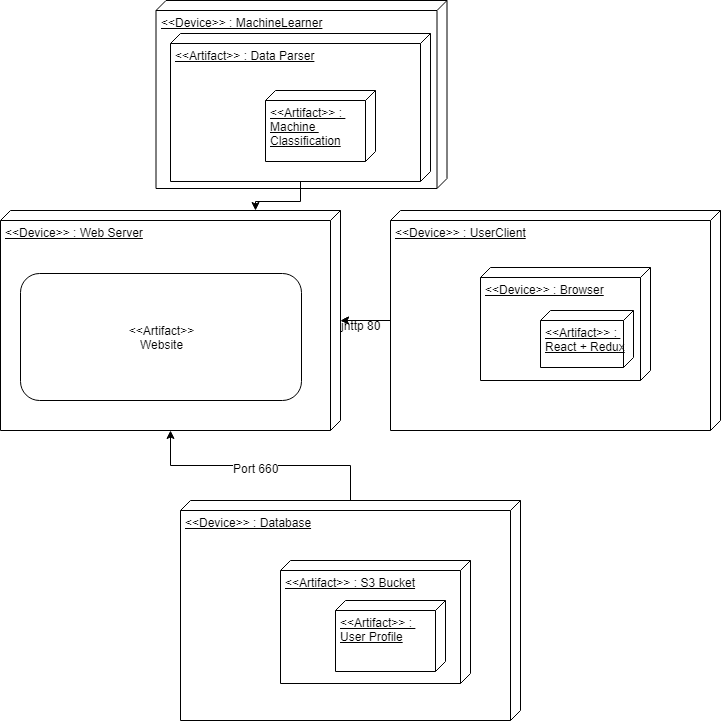
\includegraphics[scale = 0.70]{bread_deployment_diagram.png}
\begingroup
\endgroup
(See section 2.5 for details.)

\section{Issues List}
\begin{itemize}
    \item Example Ticket 1
    \begin{itemize}
        \item Example description
    \end{itemize}
    \item Example Ticket 2
    \begin{itemize}
        \item Example description
    \end{itemize}
\end{itemize}

\printnoidxglossary[sort=standard]

\end{document}

